\documentclass[10pt,landscape,a4paper]{article}
\usepackage[10pt]{moresize}
\usepackage[normalem]{ulem}
\usepackage{tikz}
\usetikzlibrary{shapes,positioning,arrows,fit,calc,graphs,graphs.standard}
\usepackage[nosf]{kpfonts}
\usepackage[t1]{sourcesanspro}
\usepackage{bold-extra}
\usepackage{multicol}
\usepackage{wrapfig}
\usepackage[top=0mm,bottom=1mm,left=0mm,right=1mm]{geometry}
\usepackage[framemethod=tikz]{mdframed}
\usepackage{microtype}
\usepackage{tabularx}
\usepackage{hhline}
\usepackage{makecell}
\usepackage{mathtools}
\usepackage{graphicx}
\usepackage[export]{adjustbox}

\DeclareMathSizes{5}{5}{4}{4}

\let\oldexists\exists
\let\exists\relax
\DeclareMathOperator{\exists}{\oldexists}
\let\oldforall\forall
\let\forall\relax
\DeclareMathOperator{\forall}{\oldforall}

\usepackage{listings}

\DeclarePairedDelimiter{\ceil}{\lceil}{\rceil}
\DeclarePairedDelimiter{\abs}{\lvert}{\rvert}%

\newcommand\codeblue[1]{\textcolor{blue}{\code{#1}}}

\usepackage{lastpage}
\usepackage{datetime}
\yyyymmdddate
\renewcommand{\dateseparator}{-}
\let\bar\overline

\definecolor{myblue}{cmyk}{1,.72,0,.38}

\def\firstcircle{(0,0) circle (1.5cm)}
\def\secondcircle{(0:2cm) circle (1.5cm)}

\colorlet{circle edge}{myblue}
\colorlet{circle area}{myblue!5}

\tikzset{filled/.style={fill=circle area, draw=circle edge, thick},
  outline/.style={draw=circle edge, thick}}

\pgfdeclarelayer{background}
\pgfsetlayers{background,main}

%\everymath\expandafter{\the\everymath \color{myblue}}
%\everydisplay\expandafter{\the\everydisplay \color{myblue}}

\everymath\expandafter{\the\everymath\color{myblue}}%\scriptstyle}

\renewcommand{\baselinestretch}{.8}
\pagestyle{empty}

% \global\mdfdefinestyle{header}{%
%   linecolor=gray,linewidth=1pt,%
%   leftmargin=0mm,rightmargin=0mm,skipbelow=0mm,skipabove=0mm,
% }

% \newcommand{\header}{
%   \begin{mdframed}[style=header]
%     \footnotesize
%     \sffamily
%     ST2334 Finals Cheatsheet (\today)\\
%     adapted from~Julius Putra Tanu Setiaji,~page~\thepage~of~\pageref{LastPage}
%   \end{mdframed}
% }

\let\counterwithout\relax
\let\counterwithin\relax
\usepackage{chngcntr}

\usepackage{verbatim}

\usepackage{etoolbox}
\makeatletter
\preto{\@verbatim}{\topsep=0pt \partopsep=0pt }
\makeatother

\counterwithin*{equation}{section}
\counterwithin*{equation}{subsection}
\usepackage{enumitem}
\newlist{legal}{itemize}{10}
\setlist[legal]{label*=\arabic*.,leftmargin=2.5mm}
\setlist[itemize]{leftmargin=2.8mm}
\setlist[enumerate]{leftmargin=4mm}
\setlist{nosep}
\usepackage{minted}

\def\code#1{\texttt{#1}}

\newenvironment{descitemize} % a mixture of description and itemize
{\begin{description}[leftmargin=*,before=\let\makelabel\descitemlabel]}
  {\end{description}}

\newcommand{\descitemlabel}[1]{%
  \textbullet\ \textbf{#1}%
}
\makeatletter

\renewcommand{\section}{\@startsection{section}{1}{0mm}%
  {.1ex}%
  {.1ex}%x
  {\color{myblue}\sffamily\bfseries}}
\renewcommand{\subsection}{\@startsection{subsection}{1}{0mm}%
  {.1ex}%
  {.1ex}%x
  {\sffamily\bfseries}}
\renewcommand{\subsubsection}{\@startsection{subsubsection}{1}{0mm}%
  {.1ex}%
  {.1ex}%x
  {\rmfamily\bfseries}}



\def\multi@column@out{%
  \ifnum\outputpenalty <-\@M
  \speci@ls \else
  \ifvoid\colbreak@box\else
  \mult@info\@ne{Re-adding forced
    break(s) for splitting}%
  \setbox\@cclv\vbox{%
    \unvbox\colbreak@box
    \penalty-\@Mv\unvbox\@cclv}%
  \fi
  \splittopskip\topskip
  \splitmaxdepth\maxdepth
  \dimen@\@colroom
  \divide\skip\footins\col@number
  \ifvoid\footins \else
  \leave@mult@footins
  \fi
  \let\ifshr@kingsaved\ifshr@king
  \ifvbox \@kludgeins
  \advance \dimen@ -\ht\@kludgeins
  \ifdim \wd\@kludgeins>\z@
  \shr@nkingtrue
  \fi
  \fi
  \process@cols\mult@gfirstbox{%
    %%%%% START CHANGE
    \ifnum\count@=\numexpr\mult@rightbox+2\relax
    \setbox\count@\vsplit\@cclv to \dimexpr \dimen@-1cm\relax
    % \setbox\count@\vbox to \dimen@{\vbox to 0.7cm{\header}\unvbox\count@\vss}%
    \else
    \setbox\count@\vsplit\@cclv to \dimen@
    \fi
    %%%%% END CHANGE
    \set@keptmarks
    \setbox\count@
    \vbox to\dimen@
    {\unvbox\count@
      \remove@discardable@items
      \ifshr@nking\vfill\fi}%
  }%
  \setbox\mult@rightbox
  \vsplit\@cclv to\dimen@
  \set@keptmarks
  \setbox\mult@rightbox\vbox to\dimen@
  {\unvbox\mult@rightbox
    \remove@discardable@items
    \ifshr@nking\vfill\fi}%
  \let\ifshr@king\ifshr@kingsaved
  \ifvoid\@cclv \else
  \unvbox\@cclv
  \ifnum\outputpenalty=\@M
  \else
  \penalty\outputpenalty
  \fi
  \ifvoid\footins\else
  \PackageWarning{multicol}%
  {I moved some lines to
    the next page.\MessageBreak
    Footnotes on page
    \thepage\space might be wrong}%
  \fi
  \ifnum \c@tracingmulticols>\thr@@
  \hrule\allowbreak \fi
  \fi
  \ifx\@empty\kept@firstmark
  \let\firstmark\kept@topmark
  \let\botmark\kept@topmark
  \else
  \let\firstmark\kept@firstmark
  \let\botmark\kept@botmark
  \fi
  \let\topmark\kept@topmark
  \mult@info\tw@
  {Use kept top mark:\MessageBreak
    \meaning\kept@topmark
    \MessageBreak
    Use kept first mark:\MessageBreak
    \meaning\kept@firstmark
    \MessageBreak
    Use kept bot mark:\MessageBreak
    \meaning\kept@botmark
    \MessageBreak
    Produce first mark:\MessageBreak
    \meaning\firstmark
    \MessageBreak
    Produce bot mark:\MessageBreak
    \meaning\botmark
    \@gobbletwo}%
  \setbox\@cclv\vbox{\unvbox\partial@page
    \page@sofar}%
  \@makecol\@outputpage
  \global\let\kept@topmark\botmark
  \global\let\kept@firstmark\@empty
  \global\let\kept@botmark\@empty
  \mult@info\tw@
  {(Re)Init top mark:\MessageBreak
    \meaning\kept@topmark
    \@gobbletwo}%
  \global\@colroom\@colht
  \global \@mparbottom \z@
  \process@deferreds
  \@whilesw\if@fcolmade\fi{\@outputpage
    \global\@colroom\@colht
    \process@deferreds}%
  \mult@info\@ne
  {Colroom:\MessageBreak
    \the\@colht\space
    after float space removed
    = \the\@colroom \@gobble}%
  \set@mult@vsize \global
  \fi}
\global\let\tikz@ensure@dollar@catcode=\relax

\def\mathcolor#1#{\@mathcolor{#1}}
\def\@mathcolor#1#2#3{%
  \protect\leavevmode
  \begingroup
  \color#1{#2}#3%
  \endgroup
}

\makeatother
\setlength{\parindent}{0pt}

\setminted{tabsize=2, breaklines}
% Remove belowskip of minted
\setlength\partopsep{-\topsep}

\setlength\columnsep{1.5pt}
\setlength\columnseprule{0.1pt}

\begin{document}

\setlength{\abovedisplayskip}{0pt}
\setlength{\belowdisplayskip}{0pt}
\ssmall
\begin{multicols*}{4}
  \raggedcolumns
  \section{Basic Concepts of Probability}
  \begin{itemize}
    \item Sample space $S$ = set of\textbf{ all possible outcomes} = \textbf{sure event}, Sample space with no elements = $\varnothing$ = \textbf{null event}
    \item \textbf{Mutually exclusive/disjoint} if $A \cap B = \varnothing$
    \item \textbf{Contained}: $A \subset B \equiv B \supset A$, \textbf{all} of the elements in A are also in B.
    \item If $A \subset B$ and $B \supset A$, then $A = B$
  \end{itemize}
  \subsection{Basic Properties}
  \vspace{-2mm}
  \begin{minipage}{\columnwidth}
    \setlength\columnseprule{0pt}
    \begin{multicols*}{2}
      \begin{itemize}
        \item $A \cap A'=\varnothing$
        \item $A \cap \varnothing = \varnothing$
        \item $A \cup A' = S$
        \item $(A \cap B)' = A' \cup B'$
        \item $(A \cup B)' = A' \cap B'$
        \item $A \cup (B \cap C) = (A \cup B) \cap (A \cup C)$
        \item $A \cap (B \cup C) = (A \cap B) \cup (A \cap C)$
        \item $A \cup B = A \cup (B \cap A')$
        \item $A = (A \cap B) \cup (A \cap B')$
        \item $(A \cap B) \cup C \neq A \cap (B \cup C)$ 
      \end{itemize}
    \end{multicols*}
  \end{minipage}
  \subsection{De Morgan's Law}
  \vspace{-1mm}
  \begin{minipage}{\columnwidth}
    \setlength\columnseprule{0pt}
    \begin{multicols*}{2}
      \begin{itemize}
        \item $(\bigcup\limits_{r = 1}^{n} A_r)' = \bigcap\limits_{r=1}^{n} (A_r)'$
        \item $(\bigcap\limits_{r = 1}^{n} A_r)' = \bigcup\limits_{r=1}^{n} (A_r)'$
      \end{itemize}
    \end{multicols*}
  \end{minipage}
  \vspace{1mm}
  \subsection{Counting Methods}
  \subsubsection{Multiplication \& Addition Principle}
  \begin{itemize}
      \item \textbf{Multiplication Principal (OP1 $\wedge$ OP2):} If an operation can be performed in $n_1$ ways, and for each of these ways a second operation can be performed in $n_2$ ways, then the 2 operations can be performed together in $n_1n_2$ ways.
      \item \textbf{Addition Principal (OP1 $\vee$ OP2):} If a first procedure can be performed in $n_1$ ways, and a second procedure in $n_2$ ways, and that it is not possible to perform both together, then the number ways we can perform either the first or second procedures is $n_1+n_2$ ways
  \end{itemize}
  \subsubsection{Permutation}
  \begin{itemize}
    \item An arrangement of $r$ objects from a set of $n$ objects, $r \leq n$, order taken into consideration.
    \item $n$ distinct objects taken $r$ at a time = $_nP_r = \frac{n!}{(n - r)!}$
    \item In a circle: $(n - 1)!$
    \item Not all are distinct: $\sum_{r=1}^{k}n_k = n$, $_nP_{n_1, n_2, ..., n_k} = \frac{n!}{n_1!n_2!...n_k!}$
  \end{itemize}
  \subsubsection{Combination}
  \begin{itemize}
    \item \# of ways of selecting $r$ from $n$ objects w/o regards to order
    \item $\binom{n}{r} = _nC_r = \frac{n!}{r!(n-r)!}$, $_nC_r \times r! = _nP_r$
    \item $\binom{n}{r}$ = binom coeff of the term $a^rb^{n-r}$ in binom expansion of $(a+b)^n$:
          \begin{itemize}
            \item $\binom{n}{r} = \binom{n}{n - r}$ for $r = 0, 1, ..., n$
            \item $\binom{n}{r} = \binom{n - 1}{r} + \binom{n - 1}{r - 1}$ for $1 \leq r \leq n$
            \item $\binom{n}{r} = 0$ for $r < 0$ pr $r > n$
          \end{itemize}
  \end{itemize}
  \subsection{Relative frequency ($f_A$)}
  $f_A = \frac{n_A}{n}$, is the relative frequency of $A$ in $n$ repetitions of experiment $E$, $n_A$ = no of times that event $A$ occurred among the $n$ repetitions.
  \subsection{Axioms of Probability}
  \begin{itemize}
    \item $0 \leq Pr(A) \leq 1$
    \item $\Pr(S) = 1$
    \item If $A_1, A_2, ...$ are mutually exclusive (disjoint),\\ i.e. $A_i \cap A_j = \varnothing$ when $i \neq j$, then $\Pr(\cup_{i=1}^\infty A_i) = \sum_{i=1}^{\infty}\Pr(A_i)$ \\
          If events $A$ and $B$ are mutually exclusive, then $\Pr(A\cup B) = \Pr(A) + \Pr(B)$
  \end{itemize}
  \subsection{Properties of Probability}
  \begin{itemize}
    \item $\Pr(\varnothing) = 0$
    \item If $A_1, A_2, ..., A_n$ are mutually exclusive, then $\Pr(\cup_{i=1}^{n}A_i) = \sum_{i=1}^{n}\Pr(A_i)$
    \item $\Pr(A) = \Pr(A \cap B) + \Pr(A \cap B')$
    \item $\Pr(A \cup B) = \Pr(A) + \Pr(B) - \Pr(A \cap B)$
    \item $\Pr (A \cup B \cup C) = \Pr(A) + \Pr(B) + \Pr(C) - \Pr(A \cap B) - \Pr(B \cap C) - \Pr(A \cap C) + \Pr(A \cap B \cap C)$
    \item \textbf{The Inclusion-Exclusion Principle}\\
          $\Pr(\bigcup\limits_{i=1}^{n}A_i) = \sum\limits_{i=1}^{n} \Pr(A_i) - \sum\limits_{i=1}^{n - 1}\sum\limits_{j = i + 1}^{n} \Pr(A_i\cap A_j) + \sum\limits_{i = 1}^{n - 2} \sum\limits_{j = i + 1}^{n - 1} \sum\limits_{k = j + 1}^{n} \Pr(A_i\cap A_j\cap A_k) - ...$
  \item If $A \subset B$, then $\Pr(A) \leq \Pr(B)$
  \end{itemize}
  \subsection{Conditional Probability, $P(A\mid B)$}
  \begin{itemize}
    \item $\Pr(A\mid B) = \frac{\Pr(A\cap B)}{\Pr(B)}$, if $\Pr(A) \neq 0$
    \item For fixed $A$, $\Pr(B\mid A)$ satisfies the postulates of probability.
    \item False positive: $\Pr(\text{+} \mid \text{condition})$
    \item Points to take note of:
    \begin{enumerate}
        \item $\Pr(A|B) \neq \Pr(B|A)$
        \item $\Pr(B|A') \neq 1- \Pr(B|A)$
        \item $\Pr(A'|B) = 1 - \Pr(A|B)$
    \end{enumerate}
  \end{itemize}
  \subsubsection{Multiplication rule}
  \begin{itemize}
    \item $\Pr(A\cap B) = \Pr(A) \Pr(B\mid A) = \Pr(B)\Pr(A\mid B)$, provided $\Pr(A) > 0, \Pr(B) > 0$
    \item $\Pr(A\cap B \cap C) = \Pr(A)\Pr(B\mid A)\Pr(C\mid A\cap B)$
    \item $\Pr(A_1\cap...\cap A_n) = \Pr(A_1)\Pr(A_2\mid A_1)\Pr(A_3 \mid A_1 \cap A_2)...\Pr(A_n\mid A_1\cap ... \cap A_{n - 1})$
  \end{itemize}
  \subsubsection{The Law of Total Probability}
  \begin{itemize}
    \item Let $A_1,A_2,...,A_n$ be a partition of sample space $S$ (mutually exclusive \& exhaustive events s.t. $A_i\cap A_j = \varnothing$ for $i\neq j$ and $\cup_{i=1}^n A_i = S$).
    \item Then $\Pr(B) = \sum_{i=1}^{n}\Pr(B\cap A_i) = \sum_{i=1}^{n}\Pr(A_i)\Pr(B\mid A_i)$
    \item e.g. $\text{P}(B)=\text{P}(A)\text{P}(B|A)+\text{P}(A')\text{P}(B|A')$
  \end{itemize}
  \subsubsection{Bayes' Theorem}
  \begin{itemize}
    \item Let $A_1,A_2,...,A_n$ be a partition of $S$
    \item $\Pr(A_k\mid B) = \frac{\Pr(A_k)\Pr(B\mid A_k)}{\sum_{i=1}^{n}\Pr(A_i)\Pr(B\mid A_i)} = \frac{\Pr(A_k)\Pr(B\mid A_k)}{\Pr(B)}$, $k \in [1, n]$
  \end{itemize}

  \subsection{Independent Events}
  \begin{itemize}
    \item \textbf{Definition}: iff $\Pr(A\cap B) = \Pr(A)\Pr(B)$
  \end{itemize}
  \subsubsection{Properties}
  \begin{itemize}
    \item Suppose $\Pr(A)>0,\Pr(B)>0$, $A$ and $B$ are independent:
          \begin{itemize}
            \item $\Pr(B\mid A) = \Pr(B)$ and $\Pr(A\mid B) = \Pr(A)$
            \item $A$ and $B$ cannot be mutually exclusive if they are independent (and vice versa)
          \end{itemize}
    \item The sample space $S$ and $\varnothing$ are independent of any event
    \item If $A \subset B$, then $A$ and $B$ are dependent unless $B = S$
  \end{itemize}
  \textcolor{red}{Warning: Independent events can't be shown using Venn Diagram, so calc!!!}
  \subsubsection{Theorem}
  If $A, B$ are independent, then so are $A$ and $B'$, $A'$ and $B$, $A'$ and $B'$.
  \subsubsection{$n$ Independent Events}
  \begin{itemize}
    \item \textbf{Pairwise Independent Events}:\\
          Events $A_1,A_2,...,A_n$ are pairwise independent iff $\Pr(A_i\cap A_j) = \Pr(A_i)\Pr(A_j)$ for $i \neq j$ and $i, j = 1,...,n$
    \item \textbf{Mutually Independent}:\\
          Events $A_1,A_2,...,A_n$ are (mutually) independent iff for any subset $\{A_{i_1}, A_{i_2},...,A_{i_k}\}$ of $A_1,A_2,...,A_n$,\\
          $\Pr(A_{i_1}\cap A_{i_2}\cap ...\cap A_{i_k}) = \Pr(A_{i_1})\Pr(A_{i_2})...\Pr(A_{i_k})$
  \end{itemize}
  \subsubsection{Remarks}
  \begin{itemize}
    \item $A_1,A_2,...,A_n$ are mutually independent $\Leftrightarrow$ for any pair of events $A_j,A_k$ where $j\neq k$, the multiplication rule holds, for any 3 distinct events, the multiplication rule holds, and so on $\Pr(A_1\cap A_2\cap ... \cap A_n) = \Pr(A_1)\Pr(A_2) ...\Pr(A_n)$. In total there are $2^n - n - 1$ diff cases.
    \item Mutually independent $\Rightarrow$ pairwise independent \textbf{(not the converse)}
    \item Suppose $A_1,A_2,...,A_n$ are mutually independent events, let $B_i=A_i$ or $A_i'$, $i \in [1, n]$. Then $B_1,B_2,...,B_n$ are also mutually independent events.
  \end{itemize}

  \section{Concepts of Random Variables}
  \subsection{Equivalent Events}
  \subsubsection{Definition}
  \begin{itemize}
    \item Let $E$ be an experiment in sample space $S$. Let $X$ be an R.V. defined on $S$, and $R_x$ its range space, i.e. $X: S \rightarrow \mathbb{R}$
    \item Let $B$ be an event w.r.t. $R_X$, i.e. $B \subset R_X$
    \item Suppose $A = \{s\in S \mid X(s) \in B \}$\\
          ($A$ consists of all sample points $s$ in $S$ for which $X(s) \in B$)
    \item $A$ and $B$ are \textbf{equivalent events}, and $\Pr(B) = \Pr(A)$
  \end{itemize}
  \subsubsection{Example}
  \begin{itemize}
    \item Consider tossing a coin twice, $S = \{ HH, HT, TH, TT \}$
    \item Let $X$ be no of heads, then $R_X=\{0, 1, 2\}$
    \item $A_1=\{HH\}$ equiv $B_1=\{2\}$, $A_2=\{HT,TH\}$ equiv $B_2=\{1\}$, $A_3=\{TT\}$ equiv $B_3=\{0\}$, $A_4=\{HH,HT,TH\}$ equiv $B_4=\{2,1\}$
  \end{itemize}
  \subsection{Discrete Probability Distributions}
  \subsubsection{Discrete R.V.}
  Let $X$ be an RV. If $R_X$ is \textbf{finite or countable infinite}, $X$ is discrete RV
  \subsubsection{Probability Fn (p.f.) or Probability Mass Function (p.m.f.)}
  \begin{itemize}
    \item For a discrete R.V., each value $X$ has a certain probability $f(x)$. Such a function $f(x)$ is called the p.f (or \textbf{probability mass function}, p.m.f).
    \item The collection of pairs $(x_i, f(x_i))$ is probability distribution of $X$
    \item The probability of $X=x_i$ denoted by $f(x_i)$ must satisfy: $f(x_i) \geq 0 \forall x_i$ and $\sum_{i=1}^{\infty}f(x_i)=1$
  \end{itemize}
  \subsection{Continuous Probability Distributions}
  \subsubsection{Continuous R.V.}
  Suppose that $R_X$ is an \textbf{interval or a collection of intervals}, then $X$ is a continuous R.V.
  \subsubsection{Probability Density Function (p.d.f.)}
  \begin{itemize}
    \item Let $X$ be a continuous R.V.
    \item p.d.f. $f(x)$ is a function satisfying:
          \begin{itemize}
            \item $f(x) \geq 0 \forall x \in R_X$
            \item $\int_{R_X}^{}f(x)\D{x} = 1$ or $\int_{-\infty}^{\infty}f(x)\D{x} = 1$ as $f(x) = 0 \forall x \notin R_X$
            \item $\forall c, d : c < d$ (i.e. $(c, d) \subset R_X$),
                  $\Pr(c\leq X \leq d) = \int_{c}^{d}f(x)\D{x}$
            \item $\Pr(X=x_0)=\int_{x_0}^{x_0}f(x)dx=0$
          \end{itemize}
  \end{itemize}
  \subsubsection{Remarks}
  \begin{itemize}
    \item $\Pr(c\leq X \leq d) = \int_{c}^{d}f(x)\D{x}$ represents area under the graph of the p.d.f. $f(x)$ between $x=c$ and $x=d$
    \item $\Pr(c \leq X \leq d) = \Pr(c \leq X < d) = \Pr(c < X \leq d) = \Pr(c<X<d)$
    \item $\Pr(A) = 0$ does not necessarily imply $A = \varnothing$
    \item $R_X \in [a, b] \Rightarrow f(x) = 0 \forall x \notin [a, b]$
    \item Note that \textbf{p.d.f can be more than 1!}
  \end{itemize}
  \subsection{Cumulative Distribution Function (c.d.f.)}
  Let $X$ be an R.V., disc or cont. $F(x)$ is a c.d.f of $X$ where $F(x) = \Pr(X\leq x)$
  \subsubsection{c.d.f. for Discrete R.V.}
  \begin{itemize}
    \item $F(x) = \sum_{t\leq x}^{}f(t) = \sum_{t\leq x}^{} \Pr(X=t)$
    \item c.d.f. of a discrete R.V. is a step function
    \item \colorbox{yellow}{$\forall a, b$ s.t. $a\leq b$, $\Pr(a\leq X \leq b) = \Pr(X \leq b) - \Pr(X < a) = F(b) - F(a^-)$} where $a^-$ is the largest possible value of $X$ strictly less than $a$
  \end{itemize}
  \subsubsection{c.d.f. for Continuous R.V.}
  \begin{itemize}
    \item $F(x) = \int_{-\infty}^{x}f(t)\D{t}$
    \item $f(x) = \frac{dF(x)}{\D{x}}$ if the derivative exists
    \item $\Pr(a\leq X \leq b) = \Pr(a < X \leq b) = F(b) - F(a)$
    \item $F(x)$ is a non-decreasing function: $x_1<x_2 \Rightarrow F(x_1) \leq F(x_2)$; and $0 \leq F(x) \leq 1$
  \end{itemize}
  \subsection{Mean and Variance of an R.V.}
  \subsubsection{Expected Value / Mean / Mathematical Expectation}
  \begin{itemize}
    \item \textbf{Discrete:} $E(X) = \mu^{}_X = \sum_i^{} x_i f_X(x_i) = \sum_x^{} x f_X(x)$
    \item If $f(x) = \frac{1}{N}$ for each of the $N$ values of $x$, $E(X) = \frac{1}{N}\sum^{}_i x_i$
    \item \textbf{Continuous:} $E(X) = \mu^{}_X = \int_{-\infty}^{\infty}\textcolor{red}{x}f_X(x)\D{x}$
    \item \textbf{Remark}: The expected value exists if the sum/integral exists
  \end{itemize}
  \subsubsection{Expectation of a function of an R.V.}
  $\forall g(X)$ with p.f. $f^{}_X(x)$
  \begin{itemize}
    \item \textbf{Discrete:} $E[g(X)] = \sum_{x}^{} g(x)f^{}_X (x)$
    \item \textbf{Continuous:} $E[g(X)] = \int_{-\infty}^{\infty} g(x) f_X(x) \D{x}$
    \item Provided the sum/integral exists.
  \end{itemize}
  \subsubsection{Variance ($\sigma_X^2 = V(X)$)}
  \begin{itemize}
    \item $g(x) = (x - \mu^{}_{X})^2$, Let $X$ be an R.V. with p.f. $f(x)$
    \item $\sigma_X^2 = V(X) = E[(X-\mu^{}_X)^2]$
    \item $E[(X-\mu^{}_X)^2] = \begin{cases}
      \sum_{x}^{} (x - \mu^{}_X)^2 f_X^{}(x) & \text{if }X\text{ is discrete}   \\
      \int_{-\infty}^{\infty}(x-\mu_X^{})^2 f_X^{}(X) \D{x} & \text{if }X\text{ is continuous}
    \end{cases}$
    \item $V(X) \geq 0$, $V(X) = E(X^2) - [E(X)]^2$
    \item \textbf{Standard deviation} = $\sigma_X^{} = \sqrt{V(X)}$
  \end{itemize}
  \subsubsection{K-th moment of $X$}
  \begin{itemize}
    \item \textbf{Definition:} $E(X^k)$, use $g(x) = x^k$ in expectation of a fn
  \end{itemize}
  \subsubsection{Properties of Expectation}
  \begin{itemize}
    \item $E(aX+b) = aE(X) + b$
    \item $V(X) = E(X^2) - [E(X)]^2$
    \item $V(aX+b)=a^2V(X)$
  \end{itemize}
  \subsection{Chebyshev's Inequality}
  \begin{itemize}
    \item Let $X$ be an R.V. with $E(X) = \mu$, $V(X) = \sigma^2_{}$
    \item $\forall k > 0$, $\Pr(\abs{X-\mu} \geq k\sigma) \leq \frac{1}{k^2}$ OR $\Pr(\abs{X-\mu}<k\sigma) \geq 1 - \frac{1}{k^2}$
    \item Holds for \textbf{all} distributions with finite mean and variance
    \item Gives a \textbf{lower bound} but not exact probability.
  \end{itemize}

  \section{2D RV \& Conditional Probability Distributions}
  \subsection{2D RV Definition (Random Vector)}
  \begin{itemize}
    \item Let $E$ be experiment and $S$ sample space associated with $E$. Let $X$ and $Y$ be 2 functions each assigning a real number to each $s \in S$. $(X, Y)$ is a 2D RV
    \item \textbf{Range Space}: $R_{x, y} = \{(x,y) \mid x = X(s), y = Y(s), s \in S\}$
    \item The definition can be extended to $n$-dimensional RV (or $n$-dimensional random vector) for $X_1, X_2, ..., X_n$.
    \item $(X, Y)$ is a 2D discrete RV if the possible values of $(X(s), Y(s))$ are \textbf{finite or countable infinite}.
    \item $(X, Y)$ is a 2D continuous RV if the possible values of $(X(s), Y(s))$ can \textbf{assume all values in some region} of the Euclidean plane $\mathbb{R}^2$
  \end{itemize}
  \subsection{Joint Probability Density Function}
  \subsubsection{For Discrete RV}
  Let $(X, Y)$ be a 2D \textbf{discrete} RV. With each possible value $(x_i, y_j)$, we associate a number $f_{X, Y}(x_i, y_j)$ representing $\Pr(X=x_i, Y=y_j)$ and satisfying:
  \begin{itemize}
    \item $f_{X, Y}(x_i, y_j) \geq 0 \forall (x_i, y_j)\in R_{X, Y}$
    \item $\sum^\infty_{i=1}\sum^\infty_{j=1}f_{X,Y}(x_i,y_j) = \sum^\infty_{i=1}\sum^\infty_{j=1}\Pr(X=x_i,Y=y_j)=1$
  \end{itemize}
  The function $f_{X, Y}(x, y)$ defined $\forall (x_i, y_j) \in R_{X, Y}$ is called \textbf{joint probability function of $(X,Y)$}.

  Let $A$ be any set consisting of pairs of $(x,y)$ values, then:

  $\Pr((X,Y) \in A) = \sum\sum_{(x,y) \in A}f_{X, Y}(x,y)$

  \subsubsection{For Continuous RV}
  Let $(X, Y)$ be a 2D continuous RV assuming all values in some region R of the Euclidean plane $\mathbb{R}^2$.

  $f_{X, Y}(x, y)$ is called joint pdf if it satisfies:
  \begin{itemize}
    \item $f_{X, Y}(x, y)\geq 0 \forall (x,y) \in R_{X, Y}$
    \item $\int\int_{(x,y)\in R_{X,Y}}f_{X,Y}\,dy\,dx = 1$ or $\int_{-\infty}^{\infty}\int_{-\infty}^{\infty}f_{X,Y}(x,y)\,dy\,dx = 1$
  \end{itemize}

  \subsection{Marginal and Conditional Probability Distributions}
  \subsubsection{Marginal Probability Distributions}
  Let $(X,Y)$ be a 2D RV with joint pdf $f_{X,Y}(x,y)$. The \textbf{marginal probability distributions} of $X$ and $Y$ are:
  \begin{itemize}
    \item \textbf{Discrete}: $f_X(x)=\sum_y f_{X,Y}(x,y)$ and $f_Y(y)=\sum_x f_{X,Y}(x,y)$
    \item \textbf{Cont}: $f_X(x)=\int_{-\infty}^{\infty}f_{X,Y}(x,y)\,dy$ and $f_Y(y)=\int_{-\infty}^{\infty}f_{X,Y}(x,y)\,dx$
    \item Basically fix one of the values, then sum/integrate over the other. Gives the probabilities of various values of the variables in the subset without reference to the values of the other variables
  \end{itemize}
  \subsubsection{Conditional Distribution}
  Let $(X,Y)$ be a 2D RV with joint pdf $f_{X,Y}(x,y)$, let $f_X(x)$ and $f_Y(y)$ be the marginal probability functions of $X$ and $Y$ respectively.

  Then the \textbf{conditional distribution of $Y$ given that $X = x$}:\\
  $f_{Y\mid X}(y \mid x) = \frac{f_{X,Y}(x,y)}{f_X(x)}$, if $f_X(x) > 0$ for each $x \in$ range of $X$

  Similarly, the \textbf{conditional distribution of $X$ given $Y=y$}:\\
  $f_{X\mid Y}(x \mid y) = \frac{f_{X,Y}(x,y)}{f_Y(y)}$, if $f_Y(y) > 0$ for each $y \in$ range of $Y$

  \textbf{Remarks}:
  \begin{itemize}
    \item The conditional p.d.f (or p.f) satisfy all the requirements for a 1D p.d.f:
          \begin{itemize}
            \item For a fixed $y$, $f_{X\mid Y}(x\mid y)\geq 0$, for a fixed $x$, $f_{Y\mid X}(y \mid X) \geq 0$
            \item For discrete RV: $\sum_x f_{X\mid Y}(x\mid y) = 1$ and $\sum_y f_{Y\mid X}(y\mid x) = 1$
            \item For cont RV: $\int_{-\infty}^{\infty}f_{X\mid Y}(x\mid y)\,dx = 1$ and $\int_{-\infty}^{\infty}f_{Y\mid X}(y\mid x)\,dy = 1$
          \end{itemize}
    \item For $f_X(x)>0$, $f_{X,Y}(x,y) = f_{Y\mid X}(y\mid x)f_X(x)$. For $f_Y(y)>0$, $f_{X,Y}(x,y) = f_{X\mid Y}(x\mid y)f_Y(y)$
  \end{itemize}

  \subsection{Independent RV}
  RV $X$ and $Y$ are independent iff $f_{X,Y}(x,y) = f_X(x)f_Y(y) \forall x,y$

  This definition can be extended to RV $X_1,X_2,...,X_n$
  \begin{itemize}
    \item The product of 2 positive functions $f_X(x)$ and $f_Y(y)$ means a function which is positive on a \textbf{product space}.
    \item i.e. if $f_X(x) > 0$ for $x \in A_1$ and $f_Y(y) > 0$ for $x \in A_2$, then $f_X(x)f_Y(y) > 0$ for $(x, y) \in A_1 \times A_2$
  \end{itemize}

  \subsection{Expectation}
  \begin{itemize}
      \item $E[g(X,Y)]=
        \begin{cases}
          \sum_x\sum_y g(x,y)f_{X,Y}(x,y)                                          & \text{for Disc RV} \\
          \int_{-\infty}^{\infty}\int_{-\infty}^{\infty}g(x,y)f_{X,Y}(x,y)\,dx\,dy & \text{for Cont RV}
        \end{cases}
      $
  
      \item $\text{E}(X) = \sum_xf_X(x)$
  \end{itemize}
  \subsubsection{Covariance ($\sigma_{x,y}$)}
  Let $g(X,Y)=(X-\mu_X)(Y-\mu_Y)$.

  Let $(X,Y)$ be a bivariate RV with joint pdf $f_{X,Y}(x,y)$, then the \textbf{covariance} of $X,Y$ is $Cov(X,Y) = E[(X-\mu_X)(Y-\mu_Y)]$
  \begin{itemize}
    \item \textbf{Discrete}: $Cov(X,Y) = \sum_x\sum_y (x-\mu_X)(y-\mu_Y)f_{X,Y}(x,y)$
    \item \textbf{Cont}: $Cov(X,Y) = \int_{-\infty}^{\infty}\int_{-\infty}^{\infty}(x-\mu_X)(y-\mu_Y)f_{X,Y}(x,y)\,dx\,dy$
  \end{itemize}
  \textbf{Remarks:}
  \begin{itemize}
    \item $Cov(X,Y) = E(XY) - \mu_X\mu_Y = E(XY) - E(X)E(Y)$
    \item If $X, Y$ are independent, then $Cov(X,Y)=0$. But $Cov(X,Y) = 0 \not\Rightarrow X$ and $Y$ are independent
    \item $Cov(aX+b,cY+d)=acCov(X,Y)$
    \item $V(aX+bY) = a^2V(X)+b^2V(Y)+2abCov(X,Y)$
  \end{itemize}
  \subsubsection{Correlation Coefficient}
  $Cor(X,Y) = \rho_{X,Y} = \frac{Cov(X,Y)}{\sqrt{V(X)}\sqrt{V(Y)}}$
  \begin{itemize}
    \item $-1 \leq \rho_{X,Y} \leq 1$
    \item $\rho_{X,Y}$ = measure of degree of \textbf{linear} relationship between $X$ and $Y$
    \item If $X, Y$ are independent, then $\rho_{X,Y}=0$. But $\rho_{X,Y}=0 \not\Rightarrow$ independence
  \end{itemize}

  \section{Special Probability Distributions}
  \subsection{Discrete Uniform Distribution}
  If RV $X$ assumes the values $x_1,x_2,...,x_k$ with equal probability, then $X$ has a discrete \textbf{uniform} distribution, and the probability function is $f_X(x) = \frac{1}{k}, x=x_1,x_2,...,x_k$, and $0$ otherwise.
  \subsubsection{Mean and Variance of Discrete Uniform Distribution}
  $\mu=E(X)=\sum xf_X(x)=\frac{1}{k}\sum_{i=1}^k x_i$

  $\sigma^2 = V(X) = \sum(x-\mu)^2f_X(x) = \frac{1}{k}\sum_{i=1}^k(x_i-\mu)^2$

  $\sigma^2=E(X^2)-\mu^2 = \frac{1}{k}(\sum_{i=1}^k x_i^2)-\mu^2$

  \subsection{Bernoulli and Binomial Distribution}
  The collection of all probability distributions for different values of the param is called a \textbf{family} of probability distributions.
  \subsubsection{Bernoulli Distribution}
  \begin{itemize}
    \item A random experiment with only 2 possible outcomes.
    \item RV $X$ has a Bernoulli distribution if the probability function of $X$ is $f_X(x)=p^x(1-p)^{1-x}, x = 0, 1$ where $0<p<1$, 0 for other $X$ values.
  \end{itemize}
  \textbf{Remarks}
  \begin{itemize}
    \item $(1-p)$ is often denoted by $q$.
    \item $\Pr(X=1)=p$ and $\Pr(X=0) = 1 - p = q$
    \item $\mu = E(X) = p$ 
    \item $\sigma^2 = V(X) = p(1 - p) = pq$
  \end{itemize}
  \subsubsection{Binomial Distributions $\sim B(n, p)$}
  \begin{itemize}
    \item RV $X$ has a \textbf{Binomial} distribution with 2 parameters $n$ and $p$, if the probability function of $X$ is $\Pr(X=x) = f_X(x)=\binom{n}{x}p^xq^{n-x}$ for $x=0,1,...,n$ where $0<p<1$
    \item $X$ is the \# of successes in $n$ independent Bernoulli trials.
    \item Bernoulli distribution is a special case of Binomial distribution when $n = 1$
    \item Mean, $\mu = E(X)=np$
    \item Variance, $\sigma^2=V(X)=npq$
    \item Conditions: (1) consists of $n$ repeated Bernoulli trials, (2) Only 2 possible outcomes in each trial, (3) $\Pr(\text{success}) = p$ is constant in each trial, (4) trials are \textbf{independent}
  \end{itemize}
  \subsubsection{Negative Binomial Distribution $\sim NB(k, p)$}
  \begin{itemize}
    \item Like binomial, but trials will be repeated until a \textbf{fixed} \# of successes occur (interested in the probability of the $k$-th success occurs on the $x$-th trials)
    \item Let $X$ be a RV represents \# of trials to produce $k$ successes in a sequence of independent Bernoulli trials
    \item $\Pr(X=x)=f_X(x)=\binom{x-1}{k-1}p^kq^{x-k}$ for $x=k, k+1, k+2,...$
    \item Mean, $\mu = E(X)=\frac{k}{p}$
    \item Variance, $\sigma^2 = V(X)=\frac{(1-p)k}{p^2}$
    \item \textbf{Special case:} \# of trials required to have the first success (i.e. $k = 1$) is \textbf{Geometric} distribution ($X\sim NB(1, p) \equiv X \sim Geom(p)$)
  \end{itemize}
  \subsection{Poisson Distribution $\sim P(\lambda)$}
  \begin{itemize}
    \item R.V. $X$, \# of successes occurring during a given time interval/in a specified region
    \item $\Pr(X=x)=f_X(x)=\frac{e^{-\lambda}\lambda^x}{x!}$ for $x=0,1,2,3,...$ where $\lambda = $ average no of successes occurring in the given time interval/specified region
    \item Mean, $\mu =E(X) = \lambda$
    \item Variance, $\sigma^2 = V(X) = \lambda$
    \item \textbf{Properties:} 
        \begin{enumerate}
            \item \# of successes in one time interval/specified region are \textbf{independent} of those in any other disjoint time interval/region of space
            \item The probability of a single success during a short time interval/in a small region is \textbf{proportional} to length of time interval/size of region, and does not depend on no of successes outside this time interval/region
            \item The prob of more than one success in such a short time interval/falling in such a small region is \textbf{negligible}
        \end{enumerate}
  \end{itemize}
  \subsection{Poisson Approximation to the Binomial Distribution}
  \begin{itemize}
    \item Let $X \sim B(n, p)$, suppose that $n \rightarrow \infty$ and $p \rightarrow 0$ such that $\lambda = np$ remains a constant as $n \rightarrow\infty$, then $X$ $\approx$ Poisson distribution with parameter $np$
    \item $\lim_{\substack{p\rightarrow0\\n\rightarrow\infty}}\text{Pr}(X=x)=\frac{e^{-np}(np)^x}{x!}$
    \item If $p\rightarrow 1$, can still use Poisson distribution to approximate binomial probabilities by swapping success \& failure s.t. $p \rightarrow 0$
  \end{itemize}
  \subsection{Continuous Uniform Distribution $\sim U(a,b)$}
  \begin{itemize}
    \item RV has \textbf{uniform} distribution over interval $[a,b]$, $-\infty<a<b<\infty$, denoted by $U(a,b)$ if its p.d.f is $f_X(x)=\frac{1}{b-a}$ for $a\leq x\leq b$ and $0$ otherwise.
    \item Mean, $\mu = E(X)=\frac{a+b}{2}$
    \item Variance, $\sigma^2=V(X)=\frac{1}{12}(b-a)^2$
  \end{itemize}
  \subsection{Exponential Distribution $\sim Exp(\alpha)$}
  \begin{itemize}
    \item Continuous RV $X$ assuming all non-negative values has an exponential distribution with parameter $\alpha > 0$ if its p.d.f is $f_X(x)=\alpha e^{-\alpha x}$ for $x > 0$ and $0$ otherwise.
    \item Mean, $\mu=E(X)=\frac{1}{\alpha}$
    \item Variance, $\sigma^2=V(X)=\frac{1}{\alpha^2}$
    \item $\int_{-\infty}^{\infty}f(x)\,dx=1$
    \item p.d.f can be written in the form $f_X(x)=\frac{1}{\mu}e^{-x/\mu}$ for $x>0$ and $0$ otherwise. Then $E(X)=\mu$, $V(X)=\mu^2$
    \item $\text{Pr}(X > t) = e^{-\alpha t}$, $\text{Pr}(X \leq t) = 1 - e^{-\alpha t}$
  \end{itemize}
  \subsubsection{No Memory Property of Exponential Distribution}
  Suppose $X \sim Exp(\alpha)$ where $\alpha > 0$, then for any 2 positive numbers $s$ and $t$, $\Pr(X>s+t \mid X>s) = \Pr(X>t)$
  \subsection{Normal Distribution $\sim N(\mu, \sigma^2)$}
  RV $X$ assuming all real values, $-\infty < x < \infty$, has a normal distribution if its p.d.f is $f_X(x)=\frac{1}{\sqrt{2\pi}\sigma}exp(-\frac{(x-\mu)^2}{2\sigma^2})$ where $-\infty<x<\infty$, $-\infty<\mu<\infty$ and $\sigma > 0$
  \subsubsection{Properties}
  \begin{itemize}
    \item Graph of the distribution is bell-shaped and symmetrical about the vertical line $x=\mu$ ($\Pr(Z\geq z_\alpha) = \Pr(Z\leq-z_\alpha)=\alpha$)
    \item Max point occurs at $x=\mu$, its value is $\frac{1}{\sqrt{2\pi}\sigma}$
    \item $E(X)=\mu$, $V(X)=\sigma^2$
    \item Total area under the curve and above the horizontal axis is $1$.
    \item The normal curve approaches the horizontal axis asymptotically in either direction away from mean. 
    \item 2 normal curves are identical in shape with same $\sigma^2$, but centered around their means. 
    \item As $\sigma$ increases, the curve flattens; as $\sigma$ decreases, the curve sharpens.
    \item If $X\sim N(\mu,\sigma^2)$ and $Z=\frac{X-\mu}{\sigma}$, then $Z\sim N(0, 1)$ (standardized normal distribution), and $E(Z) = 0$ and $V(Z) = 1$\\\\
  \end{itemize}
  
  \subsection{Normal Approximation to the Binomial Distribution}
  When $np > 5$ and $nq > 5$ ($n\rightarrow\infty$, $p\rightarrow\frac{1}{2}$)

  If $X\sim B(np, npq)$, then as $n\rightarrow\infty$, $Z=\frac{X-np}{\sqrt{npq}}$ is approx. $\sim N(0,1)$
  \subsubsection{Continuity Correction (Apply when doing normal approximation)}
  \begin{itemize}
    \item $\Pr(X=k)\approx\Pr(k-\frac{1}{2}<X<k+\frac{1}{2})$
    \item $\Pr(a\leq X\leq b)\approx\Pr(a-\frac{1}{2}<X<b+\frac{1}{2})$,
          $\Pr(a<X\leq b)\approx\Pr(a+\frac{1}{2}<X<b+\frac{1}{2})$\\
          $\Pr(a\leq X<b)\approx\Pr(a-\frac{1}{2}<X<b-\frac{1}{2})$,
          $\Pr(a< X<b)\approx\Pr(a+\frac{1}{2}<X<b-\frac{1}{2})$
    \item $\Pr(X\leq c)=\Pr(0\leq X\leq c)\approx\Pr(-\frac{1}{2}<X<c+\frac{1}{2})$
    \item $\Pr(X>c)=\Pr(c<X\leq n)\approx\Pr(c+\frac{1}{2}<X<n+\frac{1}{2})$
  \end{itemize}

  \section{Sampling and Sampling Distributions}
  \subsection{Population and Sample}
  \begin{itemize}
    \item Totality of all possible outcomes is called \textbf{population}
    \item A \textbf{sample} is any subset of a population
    \item 2 kinds of population: (1) \textbf{Finite} population, consisting of a finite number of elements, (2) \textbf{Infinite} population, consisting of an infinitely (countable and uncountable) large number of elements
    \item A set of $n$ observations from a given population is called a \textbf{sample} of size $n$
    \item Each observation in population can be considered as a value of a RV with p.d.f $f_X(x)$
  \end{itemize}
  \subsection{Random Sampling}
  \subsubsection{Simple Random Sampling (SRS)}
  A SRS of $n$ members is a sample chosen in such a way that \textbf{every subset} of $n$ observations of the population has the \textbf{same probability of being selected}
  \subsubsection{Sampling from a Finite Population}
  \begin{itemize}
    \item \textbf{Sampling without replacement}: There are $\binom{N}{n}$ samples of size $n$ to be drawn from a population of size $N$ \textbf{without replacement}. Each sample has the same probability of $1/{\binom{N}{n}}$ of being selected.
    \item \textbf{Sampling with replacement}: There are $N^n$ samples of size $n$ drawn from a population of size $N$ \textbf{with replacement}. Each sample has the same probability $\frac{1}{N^n}$ of being selected.
  \end{itemize}
  \subsubsection{Sampling from an Infinite Population}
  Random if (1) In each draw all elements of the population have the \textbf{same probability of being selected}, (2) Successive draws are \textbf{independent}
  \subsubsection{Theorem}
  Let $X$ be an RV with p.d.f $f_X(x)$, $X_1,X_2,...,X_n$ be $n$ independent RV each having the same distribution as $X$.

  Then $(X_1,X_2,...,X_n)$ is called a \textbf{random sample} of size $N$ from a population with distribution $f_X(x)$.

  The joint p.d.f is $f_{X_1,X_2,...,X_n}(x_1,x_2,...,x_n)=f_{X_1}(x_1)x_{X_2}(x_2)...f_{X_n}(x_n)$
  \subsection{Sampling distribution of sample mean ($\bar{X}$)}
  \subsubsection{Statistic and Sampling Distribution}
  \textbf{Sampling distribution} = probability distribution of a statistic
  \subsubsection{Sample Mean}
  $X_1,X_2,...,X_n$ is a random sample of size $n$ $\Rightarrow$ sample mean $\bar{X} = \frac{1}{n}\sum_{i=1}^n X_i$
  \subsubsection{Theorem}
  For random samples of size $n$ taken from \textbf{infinite} population or from \textbf{finite population with replacement} having population mean $\mu$ and population standard deviation $\sigma$, $\bar{X}$ has its mean and standard deviation: $\mu_{\bar{X}}=\mu_X$ and $\sigma_{\bar{X}}^2=\frac{\sigma_X^2}{n}$, i.e. $E(\bar{X})=E(X)$ and $V(\bar{X})=\frac{V(X)}{n}$
  \subsubsection{Law of Large Number (LLN)}
  Let $X_1,X_2,...,X_n$ be a random sample of size $n$ from a population having any distribution with mean $\mu$ and \textbf{finite} population variance $\sigma^2$. Then for any $\epsilon\in\mathbb{R}$, $\Pr(\abs{\bar{X}-\mu}>\epsilon)\rightarrow 0$ as $n\rightarrow\infty$ (basically saying that as $n \rightarrow \infty, \bar{X}$ will be very close to $\mu$)
  \subsection{Central Limit Theorem}
  Let $X_1,X_2,...,X_n$ be a random sample of size $n$ from a population having any distribution with mean $\mu$, finite population variance $\sigma^2$. $\bar{X}$ is \textbf{approximately normal} with mean $\mu$ and variance $\frac{\sigma^2}{n}$ if $n$ is \textcolor{red}{sufficiently large} $(n>30)$. Hence, $Z=\frac{\bar{X}-\mu}{\sigma/\sqrt{n}}$ follows approx. $N(0,1)$
  \begin{enumerate}
      \item Central Tendency: $\mu_{\overline{X}}=\mu$, Variance: $\sigma_{\overline{X}}=\frac{\sigma}{\sqrt{n}}$
  \end{enumerate}
  \subsubsection{Theorem}
  If $X_i$, $i=1,2,...,n$ are $N(\mu,\sigma^2)$, then $\bar{X}$ is $n(\mu,\frac{\sigma^2}{n})$ regardless of the sample size $n$. (Same thing if approximately follow)
  \subsection{Sampling Distribution of the Difference of 2 Sample Means}
  \subsubsection{Theorem}
  If independent samples of sizes $n_1$ and $n_2$ (each $\geq 30$) are drawn from 2 populations, with means $\mu_1, \mu_2$, variances $\sigma_1^2, \sigma_2^2$, then the sampling distribution of the differences of means $\bar{X}_1$ and $\bar{X}_2$ is approx. normally distributed with
  \begin{minipage}{\columnwidth}
    \setlength\columnseprule{0pt}
    \begin{multicols*}{2}
      \begin{enumerate}
          \item $\mu_{\bar{X}_1-\bar{X}_2}=\mu_1-\mu_2$ 
          \item $\sigma_{\bar{X}_1-\bar{X}_2}=\sqrt{\frac{\sigma_1^2}{n_1}+\frac{\sigma_2^2}{n_2}}$
          \item $\frac{\bar{X}_1-\bar{X}_2-(\mu_1-\mu_2)}{\sqrt{\frac{\sigma_1^2}{n_1}+\frac{\sigma_2^2}{n_2}}} \sim N(0,1)$
      \end{enumerate}
    \end{multicols*}
  \end{minipage}
  \subsection{Chi-square distribution $\sim \chi^2(n)$}
  If $Y$ is RV with p.d.f $f_Y(y)=\frac{1}{2^{n/2}\Gamma(n/2)}y^{n/2-1}e^{-y/2}$ for $y>0$ and 0 otherwise, then $Y$ has a \textbf{chi-square distribution with $n$ degrees of freedom}, denoted $\chi^2(n)$, where $n\in\mathbb{Z}^+$ and $\Gamma(\cdot)$ is the gamma function
  \subsubsection{Gamma function}
  $\Gamma(n)=\int_0^\infty x^{n-1}e^{-x}\,dx=(n-1)!$ for $n \in \mathbb{Z}^+$
  \subsubsection{Properties of Chi-square Distribution}
  \begin{itemize}
    \item If $Y\sim\chi^2(n)$, then $E(Y)=n$ and $V(Y)=2n$
    \item For large $n$, $\chi^2(n)$ approx. $\sim N(n,2n)$
    \item If $Y_1,Y_2,...,Y_k$ are \textbf{independent} chi-square RV with $n_1,n_2,...,n_k$ degrees of freedom, then $Y_1+Y_2+...+Y_k$ has a chi-square distribution with $n_1+n_2+...+n_k$ degrees of freedom: $\sum_{i=1}^k Y_i \sim \chi^2(\sum_{i=1}^k n_i)$
    \item $\Pr(Y\geq\chi^2(n;\alpha))=\alpha$ where $Y\sim\chi^2(n)$. $\Pr(Y\leq\chi^2(n;1-\alpha))=\alpha$
  \end{itemize}
  \subsubsection{From Normal to Chi-square}
  \begin{itemize}
    \item $X\sim N(0,1) \Rightarrow X^2\sim\chi^2(1)$. $X\sim N(\mu,\sigma^2) \Rightarrow (\frac{X-\mu}{\sigma})^2\sim\chi^2(1)$
    \item Let $X_1,X_2,...,X_n$ be a random sample from a normal population with mean $\mu$ and var $\sigma^2$. Define $Y=\sum_{i=1}^n\frac{(X_i-\mu)^2}{\sigma^2}$, then $Y\sim\chi^2(n)$
  \end{itemize}
  \subsubsection{The sampling distribution of $\frac{(n-1)S^2}{\sigma^2}$}
  Let $X_1,X_2,...,X_n$ be a random sample from a population, then $S^2=\frac{1}{n-1}\sum_{i=1}^n(X_i-\bar{X})^2$ is the \textcolor{red}{sample variance}

  \textbf{Theorem}: If $S^2$ is the variance of a random sample of size $n$ taken from a \textbf{normal} population, then $\frac{(n-1)S^2}{\sigma^2}\sim\chi^2(n-1)$
  \subsection{The t-distribution}
  Let $Z \sim N(0,1)$ and $U \sim \chi^2(n)$. If $Z$ and $U$ are independent, and let $T=\frac{Z}{\sqrt{U/n}}$, then the RV $T$ follows the t-distribution with $n$ degrees of freedom, $\frac{Z}{\sqrt{U/n}} \sim t(n)$
  \subsubsection{The p.d.f of a t-distribution}
  $f_T(t)=\frac{\Gamma(\frac{n+1}{2})}{\sqrt{n\pi}\Gamma(\frac{n}{2})}(1+\frac{t^2}{n})^\frac{n+1}{2}$, $-\infty<t<\infty$
  \subsubsection{Properties}
  \begin{itemize}
    \item Graph of t-distribution is symmetric about the vertical axis, resembles standard normal distribution
    \item p.d.f of t-distribution is approaching p.d.f of std normal distribution when $n\rightarrow\infty$, $\lim_{n \rightarrow \infty}f_T(t) = \frac{1}{\sqrt{2\pi}}e^{-t^2/2}$
    \item $E(T)=0$ and $V(T)=\frac{n}{n-2}$ for $n > 2$
    \item \textbf{Remark:} if the random sample was selected from a normal population, then $Z\sim N(0,1)$ and $U\sim\chi^2(n-1)$, then $T=\frac{Z}{\sqrt{U/(n-1)}}\sim t_{n-1}$
  \end{itemize}
  \subsection{The F-distribution $\sim F(n_1,n_2)$}
  Let $U\sim\chi^2(n_1)$ and $V\sim\chi^2(n_2)$, then $F=\frac{U/n_1}{V/n_2}$ is called \textbf{F-distribution} with $(n_1,n_2)$ degrees of freedom.
  \subsubsection{The p.d.f of a F-distribution}
  $f_F(x)=\frac{n_1^{n_1/2}n_2^{n_2/2}\Gamma(\frac{n_1+n_2}{2})x^{n_1/2-1}}{\Gamma(\frac{n_1}{2})\Gamma(\frac{n_2}{2}) (n_1x+n_2)^{(n_1+n_2)/2}}$ for $x>0$ and $0$ otherwise.
  \begin{enumerate}
      \item $E(X) = n_2/(n_2 - 2)$, with $n_2 > 2$
      \item $V(X)=\frac{2n_2^2(n_1+n_2-2)}{n_1(n_2-2)^2(n_2-4)}$ with $n_2 > 4$
  \end{enumerate}
  \subsubsection{Theorem}
  $F\sim F(n,m)\rightarrow \frac{1}{F}\sim F(m,n)$ and $F(n_1,n_2;1-\alpha)=\frac{1}{F(n_2,n_1;\alpha)}$

  \section{Estimation based on Normal Distribution}
  Some characteristics of elements in a population can be represented by an RV $X$ with p.d.f $f_X(x;\theta)$ where the form is assumed known, values of random sample can be observed except unknown parameters $\theta$
  \subsection{Point Estimation of Mean and Variance}
  \begin{itemize}
    \item \textbf{Point estimator} is to let the value of some statistic $\hat{\theta} = \hat{\theta}(X_1,X_2,...,X_n)$ to estimate unknown parameters $\theta$
    \item \textbf{A statistic} is a function of the random sample which does not depend on any unknown parameters. (e.g. sum/max of observations)
    \item An \textbf{estimator} is the statistic used to obtain a point estimate. ($\bar{X}$ is an estimator of $\mu$. The value of $\bar{X}$, $\bar{x}$ is an estimate of $\mu$)
  \end{itemize}
  \subsubsection{Unbiased Estimator}
  \begin{itemize}
    \item A statistic $\hat{\Theta}$ is an \textbf{unbiased estimator} of the parameters $\theta$ if $E(\hat{\Theta})=\theta$
    \item $\bar{X}$ is an unbiased estimator of $\mu$
    \item $S^2=\frac{1}{n-1}\sum_{i=1}^n(X_i-\bar{X})^2$ is unbiased estimator of $\sigma^2$, i.e. $E(S^2)=\sigma^2$
  \end{itemize}
  \subsection{Interval Estimation}
  \begin{itemize}
    \item Form: $\hat{\theta}_L<\theta<\hat{\theta}_U$ where $\hat{\theta}_L$ and $\hat{\theta}_U$ depend on (1) value of the stat $\hat{\Theta}$ for a particular sample, (2) the sampling distribution of $\hat{\Theta}$
    \item $\hat{\theta}_L$ and $\hat{\theta}_U$ = lower and upper confidence limit, $\hat{\theta}$ = point estimate
    \item Seek a random interval s.t. $\Pr(\hat{\Theta}_L<\theta<\hat{\Theta}_U)=1-\alpha$
    \item The interval computed from the selected sample is $(1-\alpha)100\%$ confidence interval for $\alpha$
    \item $(1-\alpha)$ is \textbf{confidence coefficient} or \textbf{degree of confidence}
  \end{itemize}
  \subsection{Confidence Intervals for the Mean}
  \subsubsection{Known Variance Case}
  \begin{itemize}
    \item With (i) known variance, (ii) the population is normal, or $n\geq 30$
    \item $\Pr(-z_{\alpha/2} < \frac{\bar{X}-\mu}{\sigma/\sqrt{n}}<z_{\alpha/2})=\Pr(\bar{X}-z_{\alpha/2}\frac{\sigma}{\sqrt{n}}<\mu<\bar{X}+z_{\alpha/2}\frac{\sigma}{\sqrt{n}})=1-\alpha$
    \item If $\bar{X}$ is sample mean from a popn with variance $\sigma^2$, a $(1-\alpha)100\%$ confidence interval for $\mu$ is as expression inside $\Pr$ above (middle)
  \end{itemize}
  \textbf{Sample size for Estimating $\mu$}\\
  For a given margin of error $e$, \textbf{sample size} is $n\geq(z_{\alpha/2}\frac{\sigma}{e})^2$
  \subsubsection{Unknown Variance Case}
  \begin{itemize}
    \item With (i) unknown population variance, (ii) the population is normal or very close to normal, (iii) sample size is small ($n<30$)
    \item Let $T=\frac{(\bar{X}-\mu)}{S/\sqrt{n}}$ where $S^2$ is sample variance, then $T\sim t_{n-1}$.
    \item $\Pr(-t_{n-1;\alpha/2}<T<t_{n-1;\alpha/2})=$ $\Pr(\bar{X}-t_{n-1;\alpha/2}\frac{S}{\sqrt{n}}<\mu<\bar{X}+t_{n-1;\alpha/2}\frac{S}{\sqrt{n}})$ $=1-\alpha$
    \item $\bar{X}$ and $S$ are sample mean and standard deviation, a $(1-\alpha)100\%$ confidence interval for $\mu$ is as expressed inside $\Pr$ above (middle)
    \item For large $n>30$, the t-distribution approx. $N(0,1)$. Hence the confidence interval is given by $\bar{X}-z_{\alpha/2}(\frac{S}{\sqrt{n}})<\mu<\bar{X}+z_{\alpha/2}(\frac{S}{\sqrt{n}})$
  \end{itemize}
  \subsection{Confidence Intervals for the Difference between 2 Means}
  2 populations with means $\mu_1,\mu_2$, variances $\sigma_1^2, \sigma_2^2$ then $\bar{X}_1-\bar{X}_2$ is the point estimator of $\mu_1-\mu_2$
  \subsubsection{Known variance}
  \begin{itemize}
    \item When $\sigma_1^2\neq\sigma_2^2$ and (2 populations are normal or $n_1,n_2$ both $\geq 30$)
    \item $(\bar{X}_1-\bar{X}_2)\sim N(\mu_1-\mu_2,\frac{\sigma_1^2}{n_1}+\frac{\sigma_2^2}{n_2})$
    \item $\Pr\left(-z_{\alpha/2}<\frac{(\bar{X}_1-\bar{X}_2)-(\mu_1-\mu_2)}{\sqrt{\frac{\sigma_1^2}{n_1}+\frac{\sigma_2^2}{n_2}}}<z_{\alpha/2}\right)=1-\alpha$
    \item $(1-\alpha)100\%$ confidence interval for $\mu_1-\mu_2$ is\\
          $(\bar{X}_1-\bar{X}_2)-z_{\alpha/2}{\sqrt{\frac{\sigma_1^2}{n_1}+\frac{\sigma_2^2}{n_2}}}<\mu_1-\mu_2<(\bar{X}_1-\bar{X}_2)+z_{\alpha/2}{\sqrt{\frac{\sigma_1^2}{n_1}+\frac{\sigma_2^2}{n_2}}}$
  \end{itemize}
  \subsubsection{Large sample Confidence Interval for Unknown Variances}
  $\sigma_1^2,\sigma_2^2$ are unknown, $n_1,n_2$ both $\geq 30$, replace $\sigma_1^2,\sigma_2^2$ by their estimates $S_1^2, S_2^2$ in \textbf{6.4.1}
  \subsubsection{Unknown but Equal Variances}
  \begin{itemize}
    \item $\sigma_1^2=\sigma_2^2$, 2 populations are normal, $n_1,n_2$ both $\leq 30$
    \item Pooled sample variance $S_p^2=\frac{(n_1-1)S_1^2+(n_2-1)S_2^2}{n_1+n_2-2}\sim\chi^2_{n_1+n_2-2}$
    \item $T=\frac{(\bar{X}_1-\bar{X}_2)-(\mu_1-\mu_2)}{\sqrt{S_p^2\left(\frac{1}{n_1}+\frac{1}{n_2}\right)}}\sim t_{n_1+n_2-2}$
    \item $(1-\alpha)100\%$ confidence interval for $\mu_1-\mu_2$ is\\
          $(\bar{X}_1-\bar{X}_2)-t_{n_1+n_2-2;\alpha/2}S_p\sqrt{\frac{1}{n_1}+\frac{1}{n_2}}<\mu_1-\mu_2$\\
          $<(\bar{X}_1-\bar{X}_2)+t_{n_1+n_2-2;\alpha/2}S_p\sqrt{\frac{1}{n_1}+\frac{1}{n_2}}$
  \end{itemize}
  \subsubsection{Unknown but Equal Variances for Large Samples}
  For $n_1,n_2$ both $\geq 30$, replace $t_{n_1+n_2-2;\alpha/2}$ by $z_{\alpha/2}$ in \textbf{6.4.3}
  \subsubsection{C.I. for the Difference between 2 Means for Paired (Dependent) Data}
  \begin{itemize}
    \item E.g. same individual before and after (related observations)
    \item Point estimate of $\mu_D=\mu_1-\mu_2$ is given by $\bar{d}=\frac{1}{n}\sum_{i=1}^nd_i=\frac{1}{n}\sum_{i=1}^n(x_i-y_i)$
    \item Point estimate of $\sigma^2_D$ is given by $s_D^2=\frac{1}{n-1}\sum_{i=1}^n(d_i-\bar{d})^2$
    \item \textbf{Small sample, approximate normal population}:\\
          $T=\frac{\bar{d}-\mu_D}{s_d/\sqrt{n}}\sim t_{n-1}$\\
          $(1-\alpha)100\%$ CI for $\mu_D$ = $\bar{d}-t_{n-1;\alpha/2}(\frac{S_D}{\sqrt{n}})<\mu_D<\bar{d}+t_{n-1;\alpha/2}(\frac{S_D}{\sqrt{n}})$
    \item \textbf{For large sample ($n>30$)}, CI = $\overline{d}-z_{\alpha/2}(\frac{S_D}{\sqrt{n}})<\mu_D<\overline{d}+z_{\alpha/2}(\frac{S_D}{\sqrt{n}})$

  \end{itemize}
  \subsection{C.I. for Variances and Ratio of Variances}
  \subsubsection{C.I. for a Variance of a Normal Population}
  Sample var $S^2=\frac{1}{n-1}\sum_{i=1}^n(X_i-\bar{X})^2=\frac{1}{n-1}(\sum_{i=1}^nX_i^2-n\bar{X}^2)$ is pt est of $\sigma^2$

  \textbf{CI when $\mu$ is known}: $\frac{\sum_{i=1}^n(X_i-\mu)^2}{\chi^2_{n;\alpha/2}}<\sigma^2<\frac{\sum_{i=1}^n(X_i-\mu)^2}{\chi^2_{n;1-\alpha/2}}$

  \textbf{CI when $\mu$ is unknown}: $\frac{(n-1)S^2}{\chi^2_{n-1;\alpha/2}}<\sigma^2<\frac{(n-1)S^2}{\chi^2_{n-1;1-\alpha/2}}$

  \subsubsection{C.I. for the Ratio of 2 Variances of Norm Population with Unknown Means}
  $\frac{S_1^2}{S_2^2}\frac{1}{F_{n_1-1,n_2-1;\alpha/2}}<\frac{\sigma_1^2}{\sigma_2^2}<\frac{S_1^2}{S_2^2}F_{n_2-1,n_1-1;\alpha/2}$

  \section{Hypotheses Testing based on Normal Distribution}
  \subsection{Null and Alternative Hypotheses}
\begin{itemize}
    \item Null Hypothesis, $H_0$: Hypothesis formulated with the hope of rejecting, which leads to acceptance of the alternative hypothesis, $H_1$
    \item When we reject a hypothesis, we conclude that it is false. But if we accept it, it merely means we have insufficient evidence to believe otherwise.
    \item We often choose to state the hypothesis in a form that hopefully will be rejected, i.e. usually $H_0$ will be the status quo.
\end{itemize}
  
  \subsubsection{Types of errors}
  \begin{itemize}
    \item \textbf{Type I} (serious): $\Pr($Reject $H_0\mid H_0$ is true$)=\alpha=$ level of significance
    \item \textbf{Type II}: $\Pr($Do not reject $H_0\mid H_0$ is false$)=\beta$, Power of a test = $1-\beta$\\
  \end{itemize}
  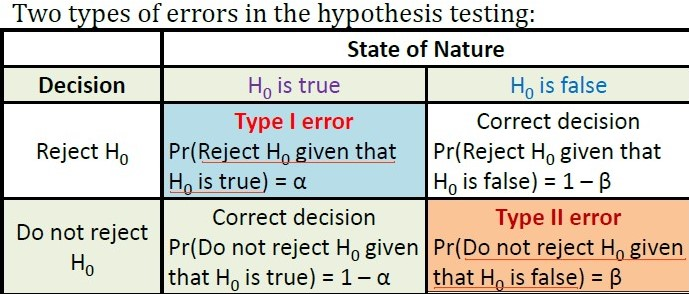
\includegraphics[scale=0.35, center]{error.jpg}\\
  \subsubsection{Acceptance and Rejection Regions}
  Rejection (critical) region and acceptance region are separated by \textbf{critical value}
  \subsection{Hypotheses Testing Concerning Mean}
  \subsubsection{Hypo Testing on Mean with Known Variance}
  Variance $\sigma^2$ is known and underlying distribution is normal or $n>30$

  \textbf{Two-sided test}:
  \begin{itemize}
    \item Test $H_0: \mu=\mu_0$ against $H_1: \mu\neq\mu_0$. Under $H_0$, we have $\bar{X}\sim N(\mu_0,\frac{\sigma^2}{n})$
    \item $\bar{x}_1<\bar{X}<\bar{x}_2$ or $-z_{\alpha/2}<Z<z_{\alpha/2}$ defines acceptance region.
    \item The two tails, $\overline{X}<\overline{x}_1$ and $\overline{X}>\overline{x}_2$ constitute the critical or rejection region.
    \item $\bar{x}_1 = \mu_0 - z_{\alpha/2}\frac{\sigma}{\sqrt{n}}$ and $\bar{x}_2=\mu_0 + z_{\alpha/2}\frac{\sigma}{\sqrt{n}}$
    \item If $\bar{X}$ falls in acceptance region, conclude $\mu=\mu_0$. Else reject $H_0$ \& accept $H_1$
    \item Basically, if the $(1-\alpha)100\%$ confidence interval covers $\mu_0$, null hypothesis is accepted, else it's rejected.
  \end{itemize}

  \textbf{One-sided test}:
  Test $H_0: \mu=\mu_0$ against $H_1:\mu>\mu_0$ or $H_1: \mu<\mu_0$. The rest is the same.
  \subsubsection{p-value Approach to Testing (observed level of significance)}
  \begin{itemize}
    \item \textbf{p-value}: Probability of obtaining a test statistic more extreme ($\leq$ or $\geq$) than the observed sample given $H_0$ is true.
  \end{itemize}
  Steps: 
  \begin{enumerate}
      \item Convert a sample statistic e.g. $\overline{X}$ into a test statistic e.g. Z statistic
      \item Obtain the p-value
      \item Compare the p-value with $\alpha/2$ (or $\alpha$). If p-value < $\alpha/2$ (or $\alpha$), reject $H_0$.
  \end{enumerate}
  \subsubsection{Hypo Testing on Mean with Unknown Variance}
  Variance unknown and underlying distribution is normal
  
  \textbf{Two-sided test:}
  
  Let $T=\frac{\bar{X}-\mu_0}{S/\sqrt{n}}$ where $S^2$ is sample variance.Reject $H_0$ if $>t_{n-1;\alpha/2}$ or $<-t_{n-1;\alpha/2}$
  
  \textbf{One-sided test:}
  
  Test the relevant side, $t>t_{n-1;\alpha}$ or $t<-t_{n-1;\alpha}$
  \subsection{Hypo Testing Concerning Difference Between 2 Means}
  \subsubsection{Known Variances}
  Known variances, normal distribution, or $n_1,n_2$ both $\geq 30$, use section 6.4.1. Generally, since variance is known, we will use $Z$ distribution.
  \subsubsection{Large Sample Testing with Unknown Variances}
  Unknown variances, both $n_1,n_2$ both $\geq 30$, use section 6.4.2
  \subsubsection{Unknown but Equal Variances}
  $\sigma_1^2=\sigma_2^2$, populations are normal, $n_1,n_2$ both $\leq 30$, use section 6.4.3
  \subsubsection{Paired Data}
  Use section 6.4.5
  \subsection{Hypo Testing Concerning Variance}
  \subsubsection{One Variance Case}
  \begin{itemize}
    \item Assume normal distribution where $\sigma^2$ is unknown.
    \item $H_0: \sigma^2=\sigma_0^2$, use test statistic: $\chi^2=\frac{(n-1)S^2}{\sigma_0^2}\sim\chi^2(n-1)$
    \item Reject $H_0$ if within critical region:\\
          \begin{tabular}{|c|c|}
            \hline
            $H_1$                    & \textbf{Critical Region}                                           \\ \hline
            $\sigma^2>\sigma_0^2$    & $\chi^2>\chi^2_{n-1;\alpha}$                                       \\ \hline
            $\sigma^2<\sigma_0^2$    & $\chi^2<\chi^2_{n-1;1-\alpha}$                                     \\ \hline
            $\sigma^2\neq\sigma_0^2$ & $\chi^2<\chi^2_{n-1;1-\alpha/2}$ or $\chi^2>\chi^2_{n-1;\alpha/2}$ \\ \hline
          \end{tabular}
  \end{itemize}
  \subsubsection{Hypo Testing Concerning Ratio of Variances}
  \begin{itemize}
    \item Assume normal distribution, unknown mean.
    \item $H_0: \sigma_1^2=\sigma_2^2$, use test statistic: $F=\frac{S_1^2}{S_2^2} \sim F(n_1 - 1, n_2-1)$
    \item Reject $H_0$ if within critical region:\\
          \begin{tabular}{|c|c|}
            \hline
            $H_1$                      & \textbf{Critical Region}                                       \\ \hline
            $\sigma_1^2>\sigma_2^2$    & $F>F_{n_1-1,n_2-1;\alpha}$                                     \\ \hline
            $\sigma_1^2<\sigma_2^2$    & $F<F_{n_1-1,n_2-1;1-\alpha}$                                     \\ \hline
            $\sigma_1^2\neq\sigma_2^2$ & $F<F_{n_1-1,n_2-1;1-\alpha/2}$ or $F>F_{n_1-1,n_2-1;\alpha/2}$ \\ \hline
          \end{tabular}
  \end{itemize}
\end{multicols*}
\end{document}
